\documentclass[]{ximera}
%handout:  for handout version with no solutions or instructor notes
%handout,instructornotes:  for instructor version with just problems and notes, no solutions
%noinstructornotes:  shows only problem and solutions

%% handout
%% space
%% newpage
%% numbers
%% nooutcomes

%I added the commands here so that I would't have to keep looking them up
%\newcommand{\RR}{\mathbb R}
%\renewcommand{\d}{\,d}
%\newcommand{\dd}[2][]{\frac{d #1}{d #2}}
%\renewcommand{\l}{\ell}
%\newcommand{\ddx}{\frac{d}{dx}}
%\everymath{\displaystyle}
%\newcommand{\dfn}{\textbf}
%\newcommand{\eval}[1]{\bigg[ #1 \bigg]}

%\begin{image}
%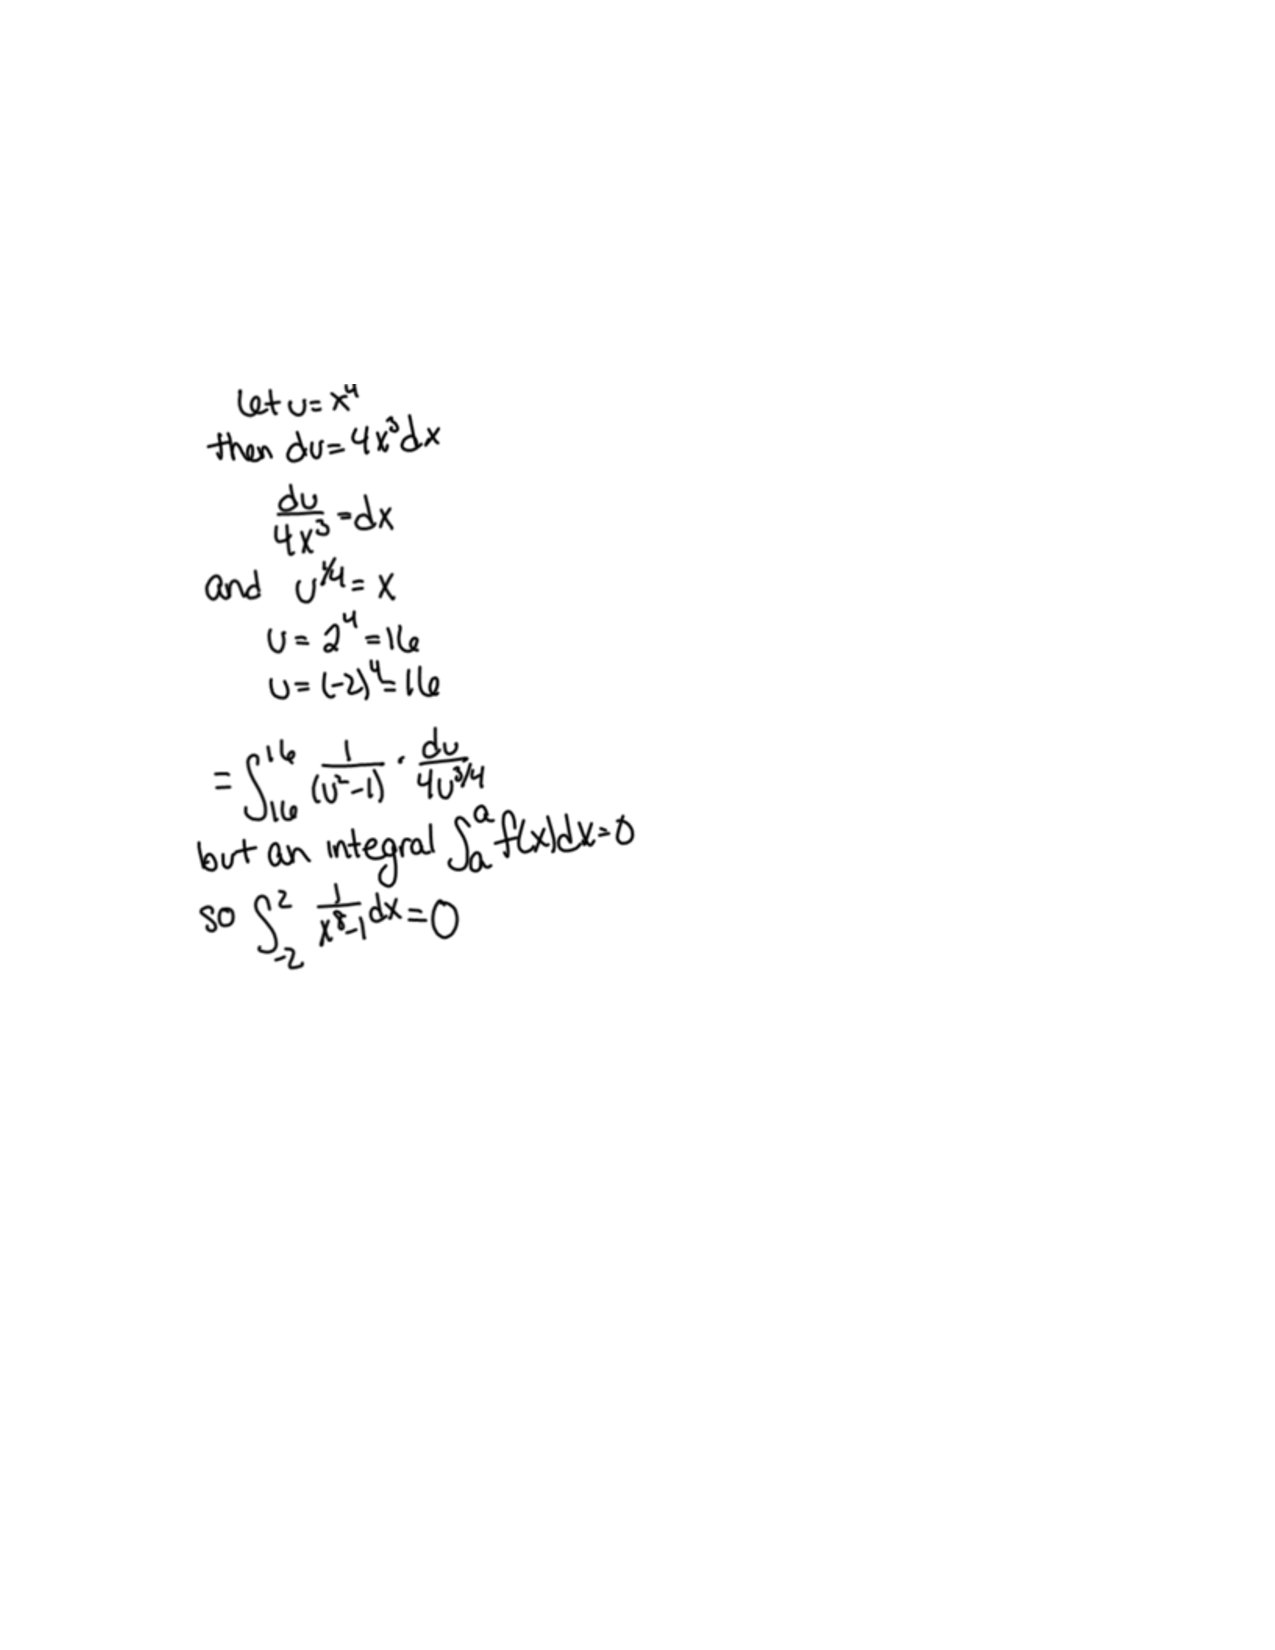
\includegraphics[trim= 170 420 250 180]{Figure1.pdf}
%\end{image}

%add a ``.'' below when used in a specific directory.
\newcommand{\RR}{\mathbb R}
\renewcommand{\d}{\,d}
\newcommand{\dd}[2][]{\frac{d #1}{d #2}}
\renewcommand{\l}{\ell}
\newcommand{\ddx}{\frac{d}{dx}}
\newcommand{\dfn}{\textbf}
\newcommand{\eval}[1]{\bigg[ #1 \bigg]}

\usepackage{multicol}

\renewenvironment{freeResponse}{
\ifhandout\setbox0\vbox\bgroup\else
\begin{trivlist}\item[\hskip \labelsep\bfseries Solution:\hspace{2ex}]
\fi}
{\ifhandout\egroup\else
\end{trivlist}
\fi} %% we can turn off input when making a master document

\title{Working with Taylor series}  

\begin{document}
\begin{abstract}		\end{abstract}
\maketitle



\section{Warm up:}
True or False:  To approximate $\frac{\pi}{3}$, one could substitute $x = \sqrt{3}$ into the Maclaurin series for $\tan^{-1}x$?
	\begin{freeResponse}
	{\bf False.}  The power series representation 
		\[
		\arctan(x) = \sum_{k=0}^\infty \frac{(-1)^k x^{2k+1}}{2k+1}
		\]
	only converges on $[-1,1]$.  
	Since $\sqrt{3}$ is outside of the IOC, one cannot substitute $x=\sqrt{3}$ into this series to approximate $\frac{\pi}{3}$.  
	\end{freeResponse}	
\begin{instructorNotes}
%There were no instructor notes for this handout.
\end{instructorNotes}







\section{Group work:}



%problem 1
\begin{problem}
Use power series to evaluate the limit
	\[
	\lim_{x \to 0} \frac{\ln (1+x^2)}{1 - \cos x}
	\]
	
	\begin{freeResponse}
	For $-1 < x \leq 1$, we know that
		\[
		\ln(1+x^2) = \sum_{k=1}^\infty \frac{(-1)^{k+1} (x^2)^k}{k} = \sum_{k=1}^\infty \frac{(-1)^{k+1} x^{2k}}{k}.
		\]
	For $- \infty < x < \infty$ we also know that
		\[
		\cos x = \sum_{k=0}^\infty \frac{(-1)^k x^{2k}}{(2k)!}.
		\]
	Since $0$ is within both of these intervals, we can substitute these formulas into the limit:
		\begin{align*}
		\lim_{x \to 0} \frac{\ln (1+x^2)}{1 - \cos x}
		&= \lim_{x \to 0} \frac{\sum_{k=1}^\infty \frac{(-1)^{k+1} x^{2k}}{k}}{1 - \sum_{k=0}^\infty \frac{(-1)^k x^{2k}}{(2k)!}}  \\
		&= \lim_{x \to 0} \frac{x^2 - \frac{x^4}{2} + \frac{x^6}{3} - \hdots}{1 - \left( 1 - \frac{x^2}{2!} + \frac{x^4}{4!} - \hdots \right)}  \\
		&= \lim_{x \to 0} \frac{x^2 - \frac{x^4}{2} + \frac{x^6}{3} - \hdots}{\frac{x^2}{2!} - \frac{x^4}{4!} + \hdots}  \\
		&= \lim_{x \to 0} \frac{x^2 \left( 1 - \frac{x^2}{2} + \frac{x^4}{3} - \hdots \right) }{x^2 \left( \frac{1}{2!} - \frac{x^2}{4!} + \hdots \right)}  \\
		&= \lim_{x \to 0} \frac{1 - \frac{x^2}{2} + \frac{x^4}{3} - \hdots }{\frac{1}{2!} - \frac{x^2}{4!} + \hdots }  \\
		= \frac{1}{\frac{1}{2}} = \boxed{2}.
		\end{align*} 
		
	\end{freeResponse}
	
\end{problem}

\begin{instructorNotes}

\end{instructorNotes}







%problem 2
\begin{problem}
Given that
	\[
	f(t) = \int_0^t x^2 \tan^{-1}(x^4) \d x
	\]
approximate $f \left( \frac{1}{3} \right)$ with the first four non-zero terms of a power series.  
Estimate how close this approximation is.
	
	\begin{freeResponse}
	
	\end{freeResponse}
		
\end{problem}

\begin{instructorNotes}

\end{instructorNotes}







%problem 3
\begin{problem}
Identify the function represented by the power series
	\[
	\sum_{k=0}^\infty \frac{k(k-1)x^4}{7^k}
	\]
	
	\begin{freeResponse}
	
	\end{freeResponse}

\end{problem}

\begin{instructorNotes}

\end{instructorNotes}







%problem 4
\begin{problem}
Use power series to determine a (series) solution to the initial value problem
	\[
	y'' - xy' + y = 0 	\qquad	y(0) = 1 	\qquad	y'(0) = 0
	\]
	
	\begin{freeResponse}
	
	\end{freeResponse}

\end{problem}

\begin{instructorNotes}

\end{instructorNotes}
















	
	
	
	
	
	
	
	
	

	










								
				
				
	














\end{document} 


















